\documentclass[a4paper,12pt,doube]{scrartcl}
%\documentclass{article}
\usepackage[english]{babel}
\usepackage[utf8]{inputenc}
\usepackage{wasysym}% provides \ocircle and \Box
%\usepackage{enumitem}% easy control of topsep and leftmargin for lists
\usepackage[inline]{enumitem}
%\usepackage{paralist}
\usepackage{color}% used for background color
\usepackage{forloop}% used for \Qrating and \Qlines
\usepackage{ifthen}% used for \Qitem and \QItem
\usepackage{graphicx} % For including graphics.
\usepackage{csquotes}
%\usepackage{typearea}
%\areaset{17cm}{26cm}
%\setlength{\topmargin}{-1cm}
\usepackage{scrlayer-scrpage}
\usepackage{cancel}
\usepackage{soul}
%\pagestyle{scrheadings}	
%\ihead{Example questionnaire created with \LaTeX}
%\ohead{\pagemark}
\chead{}
\cfoot{\pagemark}
\usepackage{setspace}
\doublespacing
\usepackage[left=4cm, right=2.5cm, top=2.5cm, bottom=2.60cm]{geometry}% Do not adjust!  Margins and spacing are set as per SGS regulations
% Disabling paragraph indentation.
\setlength\parindent{0pt}
% Setting spacing between paragraphs
\setlength\parskip{0.5\baselineskip}


%%%%%%%%%%%%%%%%%%%%%%%%%%%%%%%%%%%%%%%%%%%%%%%%%%%%%%%%%%%%
%% Beginning of questionnaire command definitions %%
%%%%%%%%%%%%%%%%%%%%%%%%%%%%%%%%%%%%%%%%%%%%%%%%%%%%%%%%%%%%
%%
%% 2010, 2012 by Sven Hartenstein
%% mail@svenhartenstein.de
%% http://www.svenhartenstein.de
%%
%% Please be warned that this is NOT a full-featured framework for
%% creating (all sorts of) questionnaires. Rather, it is a small
%% collection of LaTeX commands that I found useful when creating a
%% questionnaire. Feel free to copy and adjust any parts you like.
%% Most probably, you will want to change the commands, so that they
%% fit your taste.
%%
%% Also note that I am not a LaTeX expert! Things can very likely be
%% done much more elegant than I was able to. If you have suggestions
%% about what can be improved please send me an email. I intend to
%% add good tipps to my website and to name contributers of course.
%%
%% 10/2012: Thanks to karathan for the suggestion to put \noindent
%% before \rule!

%% \Qq = Questionaire question. Oh, this is just too simple. It helps
%% making it easy to globally change the appearance of questions.
\newcommand{\Qq}[1]{\textbf{#1}}

%% \QO = Circle or box to be ticked. Used both by direct call and by
%% \Qrating and \Qlist.
\newcommand{\QO}{$\Box$}% or: $\ocircle$
\newcommand{\QC}{$\ocircle$}% or: $\ocircle$

%% \Qrating = Automatically create a rating scale with NUM steps, like
%% this: 0--0--0--0--0.
\newcounter{qr}
\newcommand{\Qrating}[1]{\QO\forloop{qr}{1}{\value{qr} < #1}{---\QO}}

%% \Qline = Again, this is very simple. It helps setting the line
%% thickness globally. Used both by direct call and by \Qlines.
\newcommand{\Qline}[1]{\noindent\rule{#1}{0.6pt}}

%% \Qlines = Insert NUM lines with width=\linewith. You can change the
%% \vskip value to adjust the spacing.
\newcounter{ql}
\newcommand{\Qlines}[1]{\forloop{ql}{0}{\value{ql}<#1}{\vskip0em\Qline{\linewidth}}}

%% \Qlist = This is an environment very similar to itemize but with
%% \QO in front of each list item. Useful for classical multiple
%% choice. Change leftmargin and topsep accourding to your taste.
\newenvironment{Qlist}{%
	\renewcommand{\labelitemi}{\QO}
	\begin{itemize}[leftmargin=1.5em,topsep=-.5em]
	}{%
	\end{itemize}
}
\newenvironment{Qlist_SO}{% SO = Single Option
	\renewcommand{\labelitemi}{\QC}
	\begin{itemize}[leftmargin=1.5em,topsep=-.5em]
	}{%
	\end{itemize}
}

%% \Qtab = A "tabulator simulation". The first argument is the
%% distance from the left margin. The second argument is content which
%% is indented within the current row.
\newlength{\qt}
\newcommand{\Qtab}[2]{
	\setlength{\qt}{\linewidth}
	\addtolength{\qt}{-#1}
	\hfill\parbox[t]{\qt}{\raggedright #2}
}

%% \Qitem = Item with automatic numbering. The first optional argument
%% can be used to create sub-items like 2a, 2b, 2c, ... The item
%% number is increased if the first argument is omitted or equals 'a'.
%% You will have to adjust this if you prefer a different numbering
%% scheme. Adjust topsep and leftmargin as needed.
\newcounter{itemnummer}
\newcommand{\Qitem}[2][]{% #1 optional, #2 notwendig
	\ifthenelse{\equal{#1}{}}{\stepcounter{itemnummer}}{}
	\ifthenelse{\equal{#1}{a}}{\stepcounter{itemnummer}}{}
	\begin{enumerate}[topsep=2pt,leftmargin=2.8em]
		\item[\textbf{\arabic{itemnummer}#1.}] #2
	\end{enumerate}
}

%% \QItem = Like \Qitem but with alternating background color. This
%% might be error prone as I hard-coded some lengths (-5.25pt and
%% -3pt)! I do not yet understand why I need them.
\definecolor{bgodd}{rgb}{0.8,0.8,0.8}
\definecolor{bgeven}{rgb}{0.9,0.9,0.9}
\newcounter{itemoddeven}
\newlength{\gb}
\newcommand{\QItem}[2][]{% #1 optional, #2 notwendig
	\setlength{\gb}{\linewidth}
	\addtolength{\gb}{-5.25pt}
	\ifthenelse{\equal{\value{itemoddeven}}{0}}{%
		\noindent\colorbox{bgeven}{\hskip-3pt\begin{minipage}{\gb}\Qitem[#1]{#2}\end{minipage}}%
		\stepcounter{itemoddeven}%
	}{%
		\noindent\colorbox{bgodd}{\hskip-3pt\begin{minipage}{\gb}\Qitem[#1]{#2}\end{minipage}}%
		\setcounter{itemoddeven}{0}%
	}
}

\newcommand\boldred[1]{\textcolor{red}{\textbf{#1}}}
\newcommand\boldblue[1]{\textcolor{blue}{\textbf{#1}}}
\newcommand\boldgreen[1]{\textcolor{green}{\textbf{#1}}}

%%%%%%%%%%%%%%%%%%%%%%%%%%%%%%%%%%%%%%%%%%%%%%%%%%%%%%%%%%%%
%% End of questionnaire command definitions %%
%%%%%%%%%%%%%%%%%%%%%%%%%%%%%%%%%%%%%%%%%%%%%%%%%%%%%%%%%%%%

\begin{document}
	
	We are creating an AI powered social media platform designed for North American university students and research industry partners. This platform will be completely free and accessible across multiple devices, including desktops, laptops, tablets, and smartphones. 
	
	The purpose of this social media platform is to foster social connections and content sharing among students and industry professionals. Users will also gain access to free courses, paid or unpaid mentorship opportunities, and research support. Additionally, the platform will provide up-to-date information on academic conferences. The platform is equipped with a machine leaning model. The model will recommend free courses, reading materials, and video tutorials tailored to your needs. 
	
	In this survey, you will review and interpret data security and use of machine learning model terms and conditions similar to those presented when signing up for popular social media platforms such as Facebook or Instagram. This study aims to examine whether the way these terms and conditions are presented affects users’ understanding of data use for machine learning development.
	
	
	\Qitem{
		\Qq{You are a }
		\begin{Qlist_SO}
			\item UNB Undergraduate Student
			\item UNB Graduate Student
			\item UNB Industry Partner Employee
			\item Other
		\end{Qlist_SO}
	}
	
	\Qitem{
		\Qq{My background is }
		\begin{Qlist_SO}
			\item Science
			\item Engineering
			\item Social Science
			\item Business
			\item Arts
			\item Other
		\end{Qlist_SO}
	}
	
	\Qitem{
		\Qq{Do you currently use computer or smart phone for internet browsing?}
			\begin{Qlist_SO}
				\item Yes
				\item No
				\item Prefer not to answer
			\end{Qlist_SO}
	}
	\Qitem{
		\Qq{Do you currently use any search engines? Example: Google, Bing, Yahoo, Baidu, etc.}
			\begin{Qlist_SO}
				\item Yes
				\item No
				\item Prefer not to answer
			\end{Qlist_SO}
	}
	\Qitem{
		\Qq{Do you currently use any social media platforms? Example: Facebook, X (formerly Twitter), Reddit, Instagram}
			\begin{Qlist_SO}
				\item Yes
				\item No
				\item Prefer not to answer
			\end{Qlist_SO}
	}
	
	\Qitem{
		\Qq{Have you ever used AI-powered tools such as ChatGPT, Grammarly, Copilot, or similar services?}
			\begin{Qlist_SO}
				\item Yes
				\item No
				\item Prefer not to answer
			\end{Qlist_SO}
	}
	
	Please review the Terms \& Conditions for this social media platform before continuing to the next question.
	
	\Qitem{
		\Qq{How satisfied are you with the format and layout of the Terms \& Conditions?}
		\begin{Qlist_SO}
			\item Very satisfied
			\item Somewhat satisfied
			\item Satisfied
			\item Neutral
			\item Somewhat dissatisfied
			\item Dissatisfied
			\item Very dissatisfied
		\end{Qlist_SO}
	}
	
	\Qitem{
		\Qq{How easy is it for you to read and understand the Terms \& Conditions?}
		\begin{Qlist_SO}
			\item Very easy
			\item Somewhat easy
			\item Easy
			\item Neutral
			\item Somewhat difficult
			\item Difficult
			\item Very difficult
		\end{Qlist_SO}
	}
	
	\Qitem{
		\Qq{How would you rate the length of the Terms \& Conditions?}
		\begin{Qlist_SO}
			\item Very short
			\item Somewhat short
			\item Short
			\item Appropriate
			\item Somewhat long
			\item Long
			\item Very long
		\end{Qlist_SO}
	}
	
	\Qitem{
		\Qq{How would you rate your understanding of the Terms \& Conditions?}
		\begin{Qlist_SO}
			\item Not at all confident
			\item Slightly confident
			\item Somewhat confident
			\item Moderately confident
			\item Confident
			\item Very confident
			\item Extremely confident
		\end{Qlist_SO}
	}	
	
%	\Qitem{
%		\Qq{Are you aware that the platform will collect your personal data while you use it?}
%		\begin{Qlist_SO}
%			\item Yes, I am aware
%			\item No, I was not aware
%			\item I need more information
%		\end{Qlist_SO}
%	}
%	
%	\Qitem{
%		\Qq{Are you aware that the platform will process your previously collected personal data?}
%			\begin{Qlist_SO}
%				\item Yes, I am aware
%				\item No, I was not aware
%				\item I need more information
%			\end{Qlist_SO}
%	}
%	
%	\Qitem{
%		\Qq{Are you aware that the platform may sell your previously collected personal data?}
%			\begin{Qlist_SO}
%				\item Yes, I am aware
%				\item No, I was not aware
%				\item I need more information
%			\end{Qlist_SO}
%	}
%	
%	\Qitem{
%		\Qq{Are you aware that the platform’s machine learning model may make biased and unfair recommendations?}
%		\begin{Qlist_SO}
%			\item Yes, I am aware
%			\item No, I was not aware
%			\item I need more information
%		\end{Qlist_SO}
%	}
	
%	\Qitem{
%		\Qq{How comfortable are you with the platform collecting your personal data during use?}
%			\begin{Qlist_SO}
%				\item Very comfortable
%				\item Somewhat comfortable
%				\item Comfortable
%				\item Neutral
%				\item Somewhat uncomfortable
%				\item Uncomfortable
%				\item Very uncomfortable
%			\end{Qlist_SO}
%	}
%	
%	\Qitem{
%		\Qq{How comfortable are you with the platform processing personal data collected earlier?}
%			\begin{Qlist_SO}
%				\item Very comfortable
%				\item Somewhat comfortable
%				\item Comfortable
%				\item Neutral
%				\item Somewhat uncomfortable
%				\item Uncomfortable
%				\item Very uncomfortable
%			\end{Qlist_SO}
%	}
%	
%	\Qitem{
%		\Qq{How concerned are you about the platform selling your previously collected personal data?}
%			\begin{Qlist_SO}
%				\item Very concerned
%				\item Somewhat concerned
%				\item Concerned
%				\item Neutral
%				\item Somewhat concerned
%				\item Not concerned
%				\item Not concerned at all
%			\end{Qlist_SO}
%	}
%	
%	\Qitem{
%		\Qq{How concerned are you about the platform’s machine learning model making biased recommendations?}
%		\begin{Qlist_SO}
%			\item Very concerned
%			\item Somewhat concerned
%			\item Concerned
%			\item Neutral
%			\item Somewhat concerned
%			\item Not concerned
%			\item Not concerned at all
%		\end{Qlist_SO}
%	}
		
%	\boldred{\Qitem{
%		\Qq{\st{What is your understanding of the Terms \& Conditions (select all that applies)?}}
%			\begin{Qlist_SO}
%				\item \st{Strongly Agree}
%				\item \st{Agree}
%				\item \st{Somewhat Agree}
%				\item \st{Neither Agree nor Disagree}
%				\item \st{Somewhat Disagree}
%				\item \st{Disagree}
%				\item \st{Strongly Disagree}
%			\end{Qlist_SO}
%	}}
	\Qitem{
		\Qq{To what extent do you agree with the following statement:\\}	
		\enquote{\textit{The platform can safeguard my personal data, including my identity and location.}}
		\begin{Qlist_SO}
			\item Strongly Agree
			\item Agree
			\item Somewhat Agree
			\item Neither Agree nor Disagree
			\item Somewhat Disagree
			\item Disagree
			\item Strongly Disagree
		\end{Qlist_SO}
	}
	
	\Qitem{
		\Qq{To what extent do you agree with the following statement:\\}
		\enquote{\textit{The underlying machine learning model will generate \textbf{fair} and \textbf{unbiased} recommendations.}}
		\begin{Qlist_SO}
		\item Strongly Agree
		\item Agree
		\item Somewhat Agree
		\item Neither Agree nor Disagree
		\item Somewhat Disagree
		\item Disagree
		\item Strongly Disagree
		\end{Qlist_SO}
	}
	
	\Qitem{
		\Qq{To what extent do you agree with the following statement:\\}
		\enquote{\textit{The platform will need my consent to process my personal data for improving existing features and developing new ones.}}
		\begin{Qlist_SO}
			\item Strongly Agree
			\item Agree
			\item Somewhat Agree
			\item Neither Agree nor Disagree
			\item Somewhat Disagree
			\item Disagree
			\item Strongly Disagree
		\end{Qlist_SO}
	}
	
	\Qitem{
		\Qq{To what extent do you agree with the following statement:\\}
		\enquote{\textit{The platform may sell my personal data it has previously collected.}}
		\begin{Qlist_SO}
			\item Strongly Agree
			\item Agree
			\item Somewhat Agree
			\item Neither Agree nor Disagree
			\item Somewhat Disagree
			\item Disagree
			\item Strongly Disagree
		\end{Qlist_SO}
	}
	
	\Qitem{
		\Qq{To what extent do you agree with the following statement:\\}
		\enquote{\textit{The platform may share your personal data such as identity, images, and location with banks, insurance companies, and law enforcement agencies.}}
		\begin{Qlist_SO}
			\item Strongly Agree
			\item Agree
			\item Somewhat Agree
			\item Neither Agree nor Disagree
			\item Somewhat Disagree
			\item Disagree
			\item Strongly Disagree
		\end{Qlist_SO}
	}
			
	\Qitem{
		\Qq{How likely are you to use the free social media platform?}
			\begin{Qlist_SO}
				\item Very likely
				\item Somewhat likely
				\item Likely
				\item Neutral
				\item Somewhat unlikely
				\item Unlikely
				\item Very unlikely
			\end{Qlist_SO}
	}
	\Qitem{
		\Qq{Do you feel you need to revisit Terms \& Conditions again?}
		\begin{Qlist_SO}
			\item TBD
			
		\end{Qlist_SO}
		}
%	\boldred{\Qitem{
%		\Qq{If you responded ‘Disagree’ or ‘Strongly Disagree’ or ‘Neither Agree nor Disagree’, please provide the reasons for your decision (select all that applies).?}
%			\begin{Qlist}
%				\item I do not agree with the Terms \& Conditions
%				\item Terms \& Conditions are vague
%				\item Other reasons
%			\end{Qlist}
%	}}
	
	Please review the information below before proceeding to the next section. The details provided will be required to continue with the remaining of this survey.
	
	\begin{figure}[h]
		\centering
		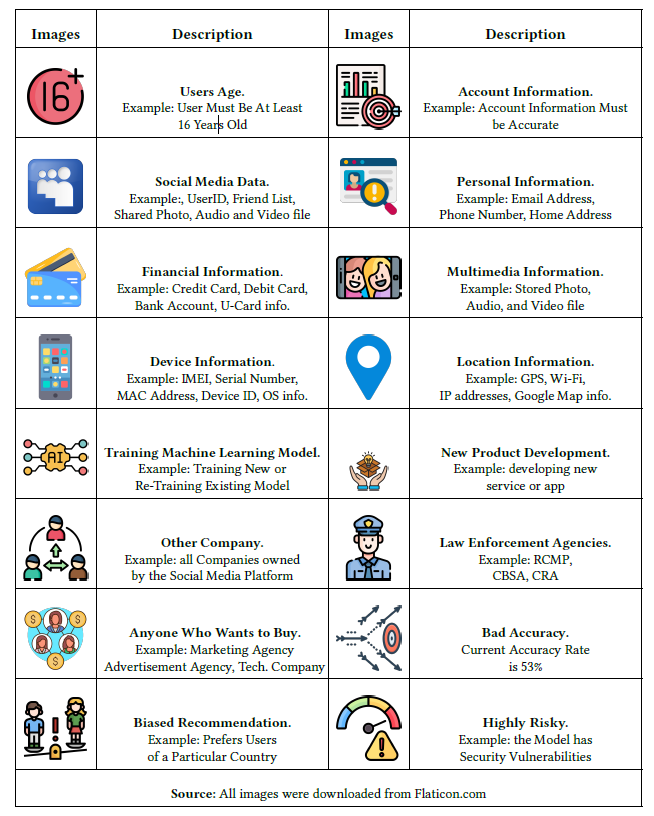
\includegraphics[width=\linewidth]{../images/VFS_Info}
		\caption{\boldred{VFS image used.}}
		\label{fig:VFS_Image}
	\end{figure}
	
	Please review the visually presented Terms \& Conditions for this social media platform before proceeding to the next question.
	
	\begin{figure}[h]
		\centering
		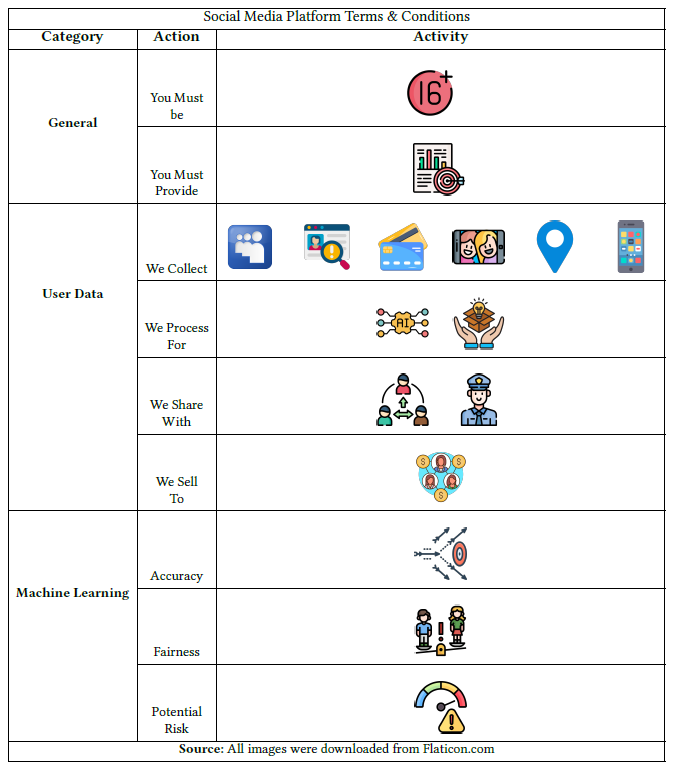
\includegraphics[width=\linewidth]{../images/VFS_main}
		\caption{\boldred{Terms \& Conditions for the Social Media Platform}}
		\label{fig:VFS}
	\end{figure}
	
	\Qitem{
		\Qq{Would you consider using the free social media platform?}
		\begin{Qlist_SO}
			\item Very likely
			\item Somewhat likely
			\item Likely
			\item Neutral
			\item Somewhat unlikely
			\item Unlikely
			\item Very unlikely
		\end{Qlist_SO}
	}
	
	{\Qitem{
		\Qq{Please provide the reasons for your decision (select all that applies).?}
		\begin{Qlist}
			\item The platform will collect my personal data
			\item The platform will sell my personal data
			\item The platform will share my personal data without my consent
			\item Machine learning model is bad
			\item Other
		\end{Qlist}
	}
		
%	\Qitem{
%		\Qq{Are the visually presented Terms \& Conditions easy for you to understand?}
%		\begin{Qlist_SO}
%			\item Very easy
%			\item Somewhat easy
%			\item Easy
%			\item Neutral
%			\item Somewhat difficult
%			\item Difficult
%			\item Very difficult
%		\end{Qlist_SO}
%	}
	
	\Qitem{
		\Qq{How effective is the visual design in helping you understand the Terms \& Conditions?}
		\begin{Qlist_SO}
			\item Not at all effective
			\item Slightly effective
			\item Somewhat effective
			\item Moderately effective
			\item Effective
			\item Very effective
			\item Extremely effective
		\end{Qlist_SO}
	}
	
%	\Qitem{
%		\Qq{Do you find the visually presented Terms \& Conditions too long, too short, or just right?}
%		\begin{Qlist_SO}
%			\item Very short
%			\item Somewhat short
%			\item Short
%			\item Appropriate
%			\item Somewhat long
%			\item Long
%			\item Very long
%		\end{Qlist_SO}
%	}
	
	\Qitem{
		\Qq{How would you rate your understanding of the Terms \& Conditions when shown in a visual format?}
		\begin{Qlist_SO}
			\item Very confident
			\item Somewhat confident
			\item Confident
			\item Neutral
			\item Not very confident
			\item Not confident
			\item Not confident at all
		\end{Qlist_SO}
	}	
		
%	\Qitem{
%		\Qq{When presented in text format, I was not aware of }
%		\begin{Qlist_SO}
%			\item Yes, I am aware
%			\item No, I was not aware
%			\item I need more information
%		\end{Qlist_SO}
%	}
	
	%	\textbf{1 Strongly disagree 2 Disagree 3 Neutral 4 Agree 5 Strongly agree}
%	\Qitem{
%		\Qq{How aware are you now that the platform collects your personal data during use?}
%		\begin{Qlist_SO}
%			\item Yes, I am aware
%			\item No, I was not aware
%			\item I need more information
%		\end{Qlist_SO}
%	}
%	
%	\Qitem{
%		\Qq{Are you aware that the platform will process your previously collected personal data?}
%		\begin{Qlist_SO}
%			\item Yes, I am aware
%			\item No, I was not aware
%			\item I need more information
%		\end{Qlist_SO}
%	}
	
%	\Qitem{
%		\Qq{Are you aware that the platform may sell your previously collected personal data?}
%		\begin{Qlist_SO}
%			\item Yes, I am aware
%			\item No, I was not aware
%			\item I need more information
%		\end{Qlist_SO}
%	}
	
	\Qitem{
		\Qq{To what extent do you agree with the following statement:\\}
		\enquote{\textit{The platform’s machine learning model may generate \textbf{biased} and \textbf{unfair} recommendations.}}
		\begin{Qlist_SO}
			\item Strongly Agree
			\item Agree
			\item Somewhat Agree
			\item Neither Agree nor Disagree
			\item Somewhat Disagree
			\item Disagree
			\item Strongly Disagree
		\end{Qlist_SO}
	}
	
	\Qitem{
		\Qq{How concerned are you with the platform collecting your personal data during use?}
		\begin{Qlist_SO}
			\item Very concerned
			\item Somewhat concerned
			\item Concerned
			\item Neutral
			\item Somewhat concerned
			\item Not concerned
			\item Not concerned at all
		\end{Qlist_SO}
	}
	
	\Qitem{
		\Qq{How concerned are you with the platform processing personal data collected earlier?}
		\begin{Qlist_SO}
			\item Very concerned
			\item Somewhat concerned
			\item Concerned
			\item Neutral
			\item Somewhat concerned
			\item Not concerned
			\item Not concerned at all
		\end{Qlist_SO}
	}
	
	\Qitem{
		\Qq{How concerned are you about the platform selling your previously collected personal data?}
		\begin{Qlist_SO}
			\item Very concerned
			\item Somewhat concerned
			\item Concerned
			\item Neutral
			\item Somewhat concerned
			\item Not concerned
			\item Not concerned at all
		\end{Qlist_SO}
	}
	
	\Qitem{
		\Qq{How concerned are you about the platform’s machine learning model making biased recommendations?}
		\begin{Qlist_SO}
			\item Very concerned
			\item Somewhat concerned
			\item Concerned
			\item Neutral
			\item Somewhat concerned
			\item Not concerned
			\item Not concerned at all
		\end{Qlist_SO}
	}
	
%	\boldred{\Qitem{
%			\Qq{\st{What is your understanding of the Terms \& Conditions (select all that applies)?}}
%			\begin{Qlist_SO}
%				\item \st{Strongly Agree}
%				\item \st{Agree}
%				\item \st{Somewhat Agree}
%				\item \st{Neither Agree nor Disagree}
%				\item \st{Somewhat Disagree}
%				\item \st{Disagree}
%				\item \st{Strongly Disagree}
%			\end{Qlist_SO}
%	}}
	
%	\boldred{\Qitem{
%			\Qq{If you responded ‘Disagree’ or ‘Strongly Disagree’ or ‘Neither Agree nor Disagree’, please provide the reasons for your decision (select all that applies).?}
%			\begin{Qlist}
%				\item I do not agree with the Terms \& Conditions
%				\item Terms \& Conditions are vague
%				\item Other reasons
%			\end{Qlist}
%	}}

	\Qitem{
			\Qq{How effective was the visual presentation of the Terms \& Conditions in explaining the platform’s data collection, processing, and sharing policies?}
			\begin{Qlist}
				\item Extremely effective
				\item Very effective
				\item Effective
				\item Moderately effective
				\item Somewhat effective
				\item Slightly effective
				\item Not at all effective
			\end{Qlist}
	}

	\Qitem{
			\Qq{To what extent did the visual design of the Terms \& Conditions improve your understanding of machine learning features on the platform?}
			\begin{Qlist}
				\item Completely
				\item Very much
				\item Considerably
				\item Moderately
				\item Somewhat
				\item Slightly
				\item Not at all
			\end{Qlist}
	}
	
%	\boldred{\Qitem{
%			\Qq{How did the visual presentation of the Terms \& Conditions help you understand the use of machining learning into the free social media platform (select all that applies)?}
%	}}
	
	\boldred{\Qitem{
			\Qq{Do you have any observations or suggestions?}
	}}

	
%	\begin{center}
%		\textbf{\huge Example questionnaire created with \LaTeX}
%	\end{center}\vskip1em
%	
%	\noindent Welcome to this very important survey with which we
%	researchers want to look deep inside of you (be afraid!). Anyway,
%	thank you for filling it all out.
%	
%	\noindent \textit{Please note that no tabular environment is used in
%		this example questionnaire. Of course, you could use tabular to
%		create more complex layout.}
%	
%	\section*{About you}
%	
%	\Qitem{ \Qq{Your name}: \Qline{8cm} }
%	
%	\Qitem{ \Qq{How old are you?} I am \Qline{1.5cm} years old.}
%	
%	\Qitem{ \Qq{Are you in a good mood right now?} \hskip0.4cm \QO{}
%		absolutely \hskip0.5cm \QO{} not really because: \Qline{3cm} }
%	
%	\Qitem{ \Qq{Do you like having an option?}
%		\begin{Qlist}
%			\item Yes, this meets my need for autonomy.
%			\item No, I'd rather have someone else decide for me.
%			\item Not sure.
%		\end{Qlist}
%	}
%	
%	\Qitem{ \Qq{What kind of music do you like best?}
%		\begin{Qlist}
%			\item Johann Sebastian Bach
%			\item Jazz
%			\item The Beatles
%			\item Other: \Qline{4cm}
%		\end{Qlist}
%	}
%	
%	\minisec{Please evaluate the following composers}
%	\vskip.5em
%	
%	\Qitem[a]{ \Qq{Mozart} \Qtab{3cm}{horrible \Qrating{5} fantastic}}
%	
%	\Qitem[b]{ \Qq{Beethoven} \Qtab{3cm}{horrible \Qrating{5} fantastic}}
%	
%	\Qitem[c]{ \Qq{Johann S. Bach} \Qtab{3cm}{horrible \Qrating{5}
%			fantastic}}
%	
%	\Qitem[d]{ \Qq{John Lennon}\Qtab{2.5cm}{\parbox[t]{3.3cm}{\raggedleft
%				Uh, well, I do not like his music very much}
%			\Qrating{7} \parbox[t]{3cm}{Oh, yes, you know, really great
%				stuff}}}
%	
%	\Qitem[e]{ \Qq{Elvis}\Qtab{2.5cm}{\parbox[t]{3.3cm}{\raggedleft Uh,
%				well, I do not like his music very much}
%			\Qrating{7} \parbox[t]{3cm}{Oh, yes, you know, really great
%				stuff}}}
%	
%	\section*{About this questionnaire}
%	
%	\Qitem{\Qq{Do you like the style so far?} \Qtab{5.5cm}{\QO{} Yes
%			\hskip0.5cm \QO{} No}}
%	
%	\Qitem{\Qq{Is it really worth the ink?} \Qtab{5.5cm}{\QO{} Guess so.
%			\hskip0.5cm \QO{} Probably not. \hskip0.5cm \QO{} Don't know.}}
%	
%	\Qitem{\Qq{How does this item look different from the previous one?}
%		\Qtab{10.5cm}{\QO{}\Qtab{0.6cm}{Oh. Does it?}}\par
%		\Qtab{10.5cm}{\QO{}\Qtab{0.6cm}{No clue. I just can't figure it out.
%				So sorry.}}\par
%		\Qtab{10.5cm}{\QO{}\Qtab{0.6cm}{I guess what you mean is that here
%				the different answer options are below each other.}}\par
%	}
%	
%	\Qitem[a]{ \Qq{Please describe your first impression.} \Qlines{2} }
%	
%	\Qitem[b]{ \Qq{In case you would like some more lines to write, here
%			they are:} \Qlines{4} }
%	
%	\section*{Another feature}
%	
%	\noindent Now, here is another nice feature: you can automatically
%	alter the background color of the items. Here is how it can look like.
%	Because we are too lazy to think of new questions we will just ask you
%	the same questions again. There is one difference to the above though,
%	can you find it?
%	
%	\renewcommand{\QO}{$\ocircle$}% Use circles now instead of boxes.
%	
%	\section*{About you}
%	
%	\QItem{ \Qq{Your name}: \Qline{8cm} }
%	
%	\QItem{ \Qq{How old are you?} I am \Qline{1.5cm} years old.}
%	
%	\QItem{ \Qq{Are you in a good mood right now?} \hskip0.4cm \QO{}
%		absolutely \hskip0.5cm \QO{} not really because: \Qline{3cm} }
%	
%	\QItem{ \Qq{Do you like having an option?}
%		\begin{Qlist}
%			\item Yes, this meets my need for autonomy.
%			\item No, I'd rather have someone else decide for me.
%			\item Not sure.
%		\end{Qlist}
%	}
%	
%	\QItem{ \Qq{What kind of music do you like best?}
%		\begin{Qlist}
%			\item Johann Sebastian Bach
%			\item Jazz
%			\item The Beatles
%			\item Other: \Qline{4cm}
%		\end{Qlist}
%	}
%	
%	\minisec{Please evaluate the following composers}
%	\vskip.5em
%	
%	\QItem[a]{ \Qq{Mozart} \Qtab{3cm}{horrible \Qrating{5} fantastic}}
%	
%	\QItem[b]{ \Qq{Beethoven} \Qtab{3cm}{horrible \Qrating{5} fantastic}}
%	
%	\QItem[c]{ \Qq{Johann S. Bach} \Qtab{3cm}{horrible \Qrating{5} fantastic}}
%	
%	\QItem[d]{ \Qq{John Lennon}\Qtab{2.5cm}{\parbox[t]{3.3cm}{\raggedleft
%				Uh, well, I do not like his music very much}
%			\Qrating{7} \parbox[t]{3cm}{Oh, yes, you know, really great
%				stuff}}}
%	
%	\QItem[e]{ \Qq{Elvis}\Qtab{2.5cm}{\parbox[t]{3.3cm}{\raggedleft
%				Uh, well, I do not like his music very much}
%			\Qrating{7} \parbox[t]{3cm}{Oh, yes, you know, really great
%				stuff}}}
%	
%	\section*{About this questionnaire}
%	
%	\QItem{\Qq{Do you like the style so far?} \Qtab{5.5cm}{\QO{} Yes
%			\hskip0.5cm \QO{} No}}
%	
%	\QItem{\Qq{Is it really worth the ink?} \Qtab{5.5cm}{\QO{} Guess so.
%			\hskip0.5cm \QO{} Probably not. \hskip0.5cm \QO{} Don't know.}}
%	
%	\QItem{\Qq{How does this item look different from the previous one?}
%		\Qtab{10.5cm}{\QO{}\Qtab{0.6cm}{Oh. Does it?}}\par
%		\Qtab{10.5cm}{\QO{}\Qtab{0.6cm}{No clue. I just can't figure it out.
%				So sorry.}}\par
%		\Qtab{10.5cm}{\QO{}\Qtab{0.6cm}{I guess what you mean is that here
%				the different answer options are below each other.}}\par
%	}
%	
%	\QItem[a]{ \Qq{Please describe your first impression.} \Qlines{2} }
%	
%	\QItem[b]{ \Qq{In case you would like some more lines to write, here
%			they are:} \Qlines{4} }

	
\end{document}